\documentclass[aspectratio=169,10pt]{beamer}

\usetheme{Madrid}
\setbeamertemplate{navigation symbols}{}
\setbeamertemplate{footline}[frame number]
\setbeamertemplate{itemize items}[circle]
\setbeamertemplate{enumerate items}[default]

\usepackage[T1]{fontenc}
\usepackage{amsmath,amssymb,bm}
\usepackage{array}
\usepackage{booktabs}
\usepackage{graphicx}
\usepackage{tikz}
\usetikzlibrary{arrows.meta,positioning,calc,shapes.geometric}
\emergencystretch=3em
\pdfstringdefDisableCommands{%
  \def\translate#1{#1}%
}

\graphicspath{{../figures/}}

\definecolor{DeepBlue}{RGB}{28,54,99}
\definecolor{MidBlue}{RGB}{48,91,150}
\definecolor{PaleBlue}{RGB}{235,241,249}
\definecolor{PaleGreen}{RGB}{235,247,239}
\definecolor{PaleOrange}{RGB}{253,242,225}
\definecolor{PaleRed}{RGB}{252,236,236}
\definecolor{DarkGreen}{RGB}{39,116,75}
\definecolor{DarkOrange}{RGB}{158,93,21}
\definecolor{DarkRed}{RGB}{150,56,56}

\setbeamercolor{structure}{fg=DeepBlue}
\setbeamercolor{palette primary}{fg=white,bg=DeepBlue}
\setbeamercolor{palette secondary}{fg=white,bg=MidBlue}
\setbeamercolor{palette tertiary}{fg=white,bg=DeepBlue!85}
\setbeamercolor{palette quaternary}{fg=white,bg=DeepBlue!70}
\setbeamercolor{section in head/foot}{fg=white,bg=DeepBlue}
\setbeamercolor{subsection in head/foot}{fg=white,bg=MidBlue}
\setbeamercolor{normal text}{fg=black,bg=white}
\setbeamercolor{background canvas}{bg=white}
\setbeamercolor{frametitle}{fg=white,bg=DeepBlue}
\setbeamercolor{title}{fg=DeepBlue}
\setbeamercolor{subtitle}{fg=black}
\setbeamercolor{block title}{fg=white,bg=DeepBlue}
\setbeamercolor{block body}{fg=black,bg=white}
\setbeamercolor{alerted text}{fg=DarkRed}
\setbeamercolor{footline}{fg=black!55}
\setbeamerfont{frametitle}{series=\bfseries,size=\Large}
\setbeamerfont{title}{series=\bfseries}
\setbeamerfont{block title}{series=\bfseries}
\setbeamerfont{footline}{size=\scriptsize}
\newcommand{\sep}{\mathrm{SEP}}
\newcommand{\rom}{\mathrm{ROM1}}
\newcommand{\nn}{\mathrm{NN}}
\newcommand{\E}{\mathbb{E}}
\newcommand{\R}{\mathbb{R}}
\newcommand{\eps}{\varepsilon}
\newcommand{\thetao}{\theta}
\newcommand{\state}{s}
\newcommand{\obs}{y}
\newcommand{\stephead}[2]{%
  \begin{block}{#1}
  #2
  \end{block}
}
\newcommand{\smallnote}[1]{%
  \vspace{0.25em}
  \begin{center}
  \parbox{0.92\linewidth}{\centering\footnotesize #1}
  \end{center}
}
\newcommand{\sourcefoot}[1]{%
  \vspace{-0.55em}
  \begin{flushleft}
  \parbox{0.96\linewidth}{\raggedright\tiny\textit{#1}}
  \end{flushleft}
}
\newcommand{\claim}[1]{%
  \begin{center}
  \parbox{0.94\linewidth}{\centering\large\bfseries #1}
  \end{center}
}
\newcommand{\softline}{\par\vspace{0.12em}\noindent{\color{DeepBlue!45}\rule{0.88\linewidth}{0.45pt}}\par\vspace{0.25em}}

\title[SEP--NN DSGE Estimation]{Bayesian Estimation of Nonlinear DSGE Models\\with Neural-Network Surrogate Solvers}
\subtitle{A Stochastic Extended Path to HMC pipeline}
\author[M. Farkas]{M\'aty\'as Farkas}
\institute[IMF]{International Monetary Fund}
\date{Computational Economics Conference \\ 30-minute talk draft}

\begin{document}

% -----------------------------------------------------------------------------
\begin{frame}
  \titlepage
  \vspace{-0.5em}
  \begin{center}
  \footnotesize Views expressed are my own and do not necessarily represent the IMF.
  \end{center}
\end{frame}

% -----------------------------------------------------------------------------
\begin{frame}{Main Takeaway First}
\claim{Estimate with a switching solution-order likelihood.}

\vspace{1.1em}
\begin{columns}[T,onlytextwidth]
\begin{column}{0.48\textwidth}
\textbf{What I do}

\softline
I start each likelihood evaluation from ROM1, switch in the learned nonlinear
correction only on validated support, and keep direct SEP as the teacher and benchmark.
\end{column}
\begin{column}{0.48\textwidth}
\textbf{Why it matters}

\softline
This puts the order of approximation inside the likelihood: cheap where the
model is locally linear, richer where the posterior asks for nonlinear dynamics.
\end{column}
\end{columns}

\smallnote{The contribution is computational and econometric: the sampler sees one differentiable target, while the solution rule switches between ROM1, ROM1+NN, and direct SEP benchmark calls.}
\end{frame}

% -----------------------------------------------------------------------------
\begin{frame}{The Intuition: Precompute the Hard Object}
\claim{A surrogate is a modern lookup table for a hard economic function.}

\vspace{0.2em}
\begin{columns}[T,onlytextwidth]
\begin{column}{0.47\textwidth}
\centering
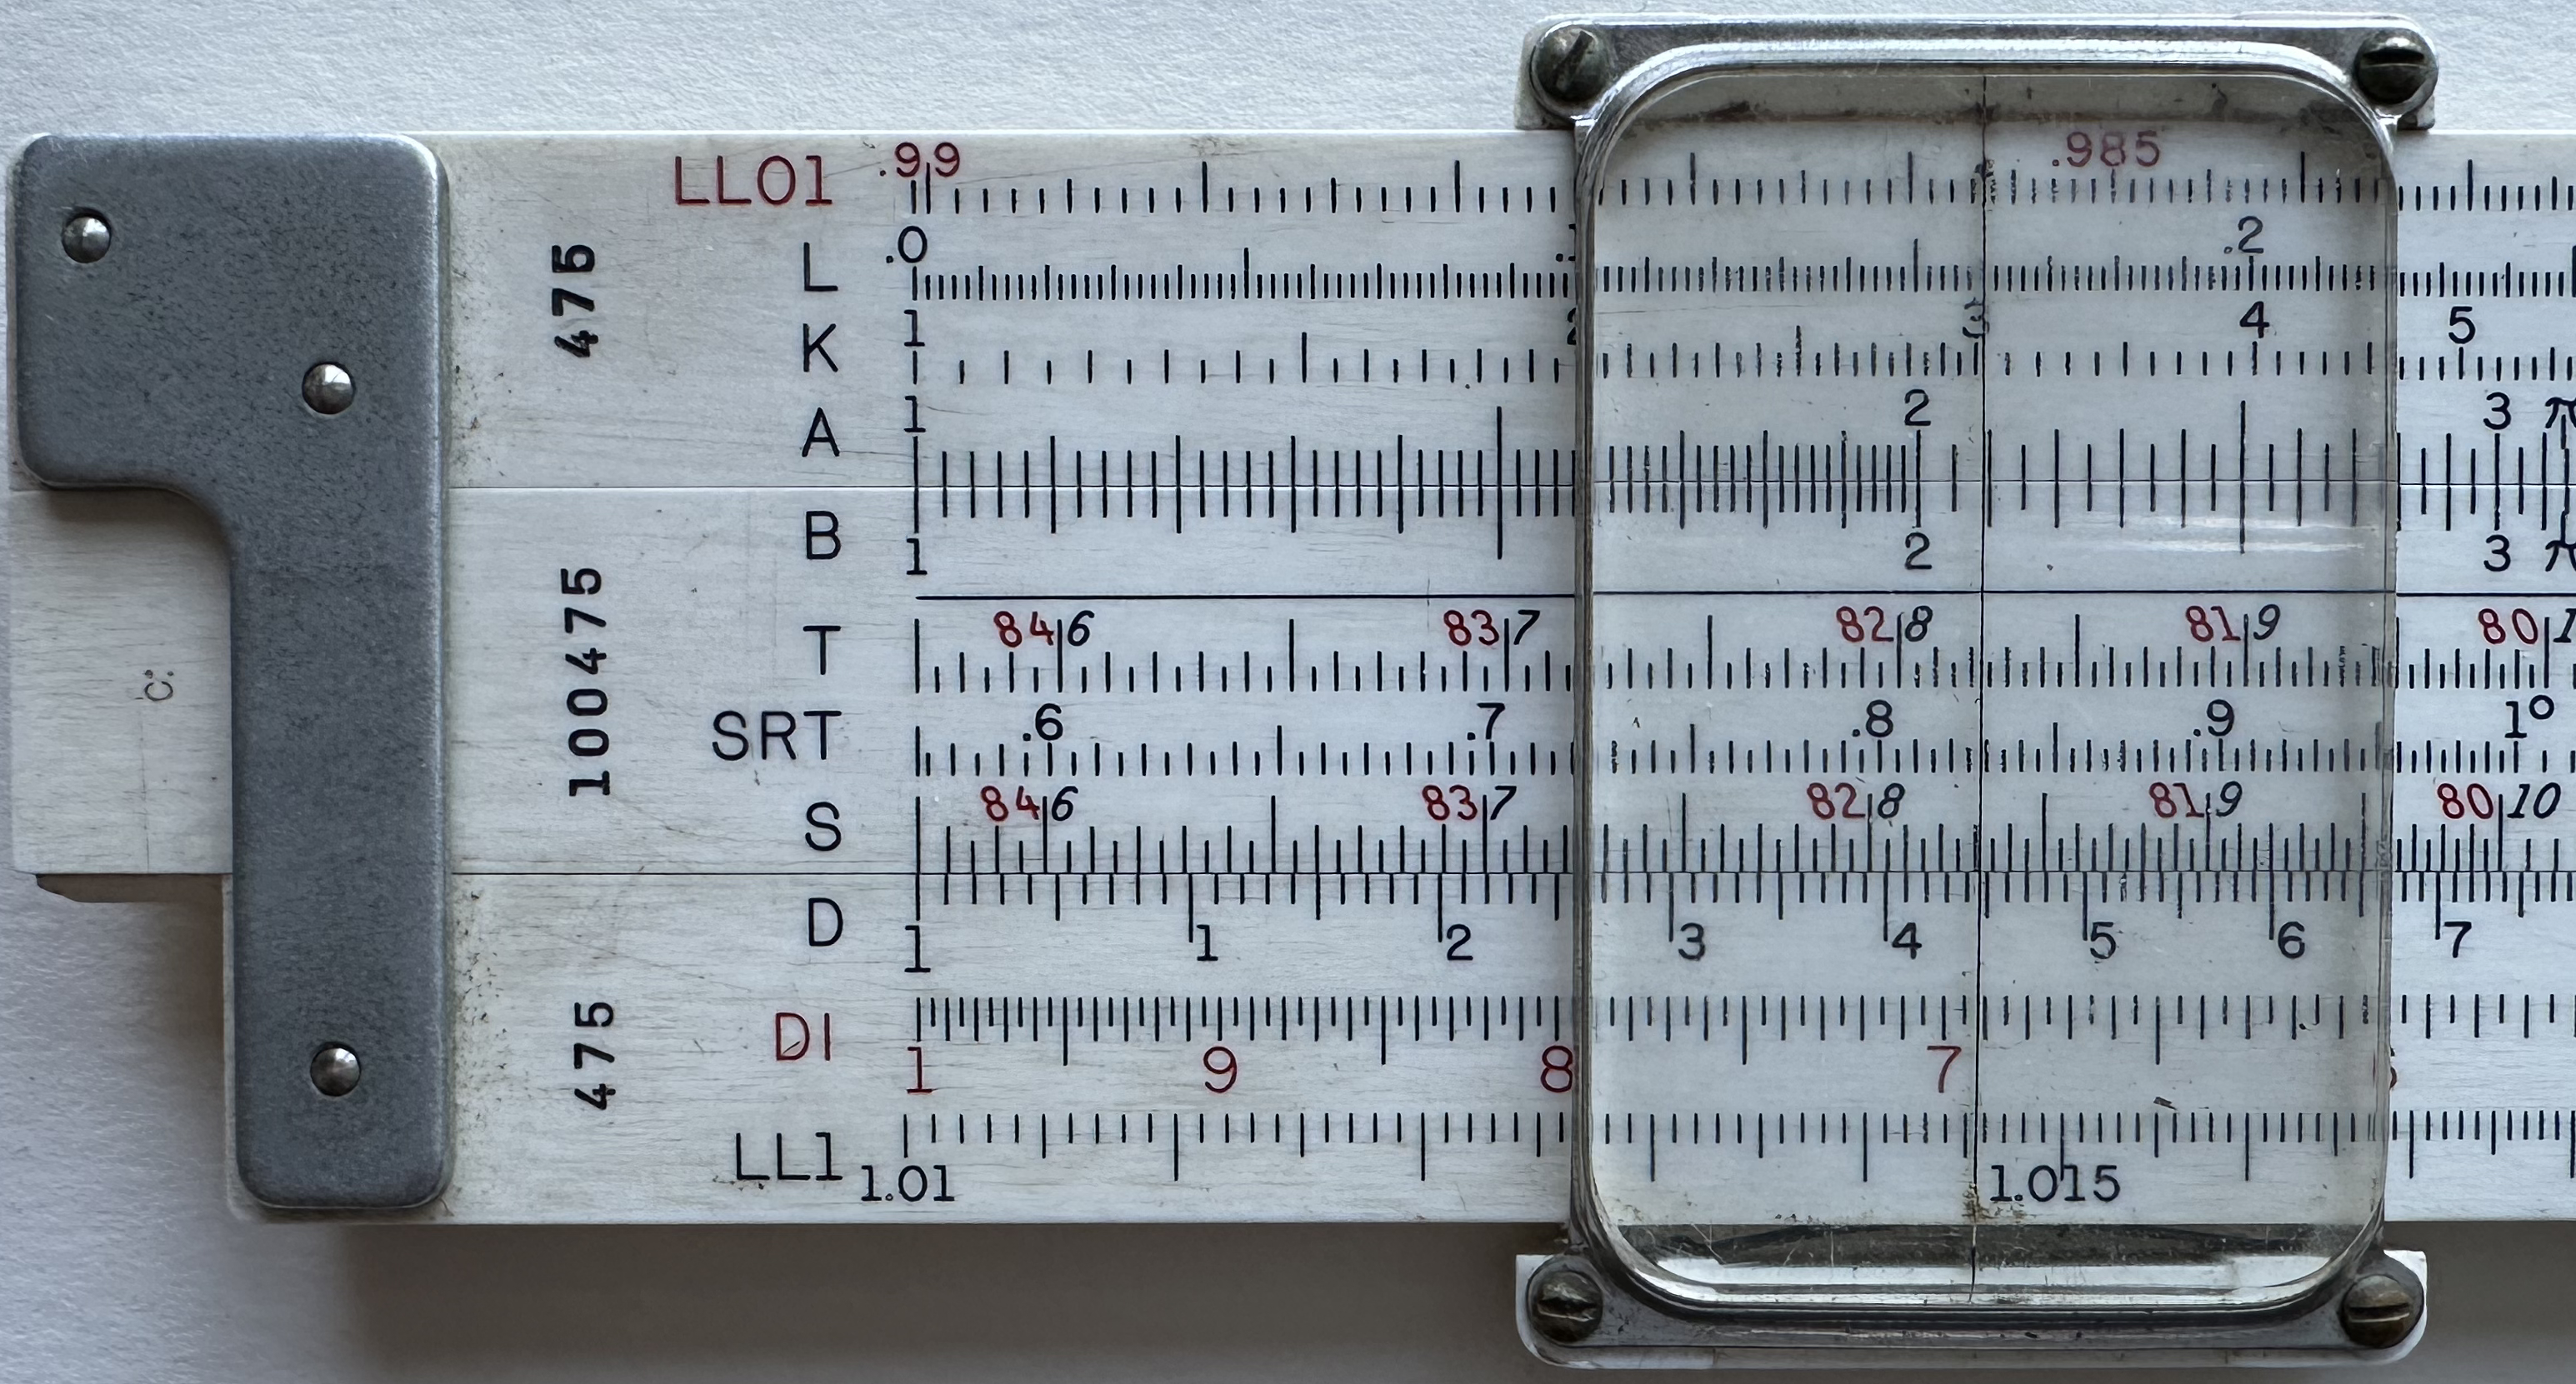
\includegraphics[width=0.92\textwidth,height=0.35\textheight,keepaspectratio]{slide_rule_scales_front.jpg}

\vspace{0.15em}
\scriptsize Logs and products were once handled by tables and interpolation.
\end{column}
\begin{column}{0.49\textwidth}
\centering
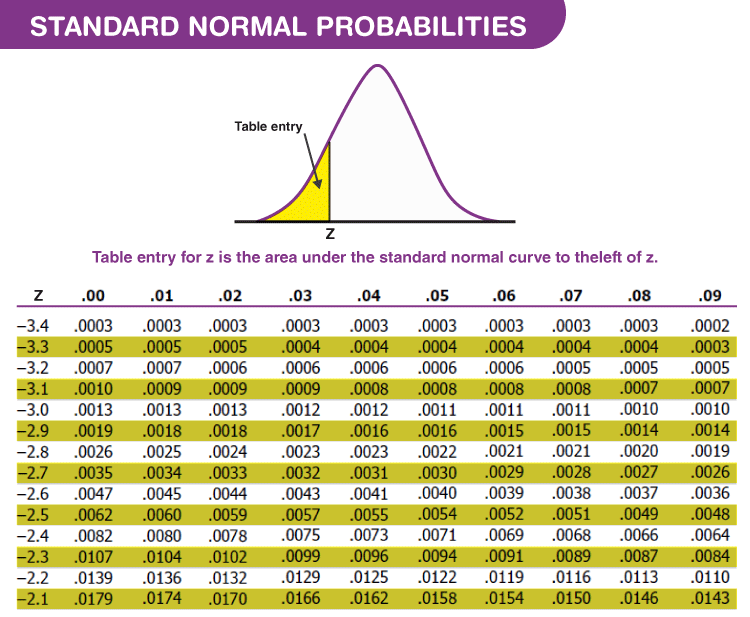
\includegraphics[width=0.83\textwidth,height=0.35\textheight,keepaspectratio]{z_score_table.png}

\vspace{0.15em}
\scriptsize Hard functions were made operational by precomputation.
\end{column}
\end{columns}

\vspace{0.55em}
\begin{center}
\normalsize
I use the same idea for a nonlinear DSGE transition map:
\[
  (\state_t,\eps_{t+1},\theta)
  \mapsto
  \state_{t+1}^{\sep}.
\]
\end{center}

\sourcefoot{Images adapted from the previous Nonlinear DSGE presentation. Slide-rule source: Arnold Reinhold, Wikimedia Commons. Z-score table source: BYJU'S.}
\end{frame}

% -----------------------------------------------------------------------------
\begin{frame}{The Hook}
\claim{Nonlinear DSGE models are economically natural and computationally awkward.}

\vspace{0.5em}
\begin{columns}[T,onlytextwidth]
\begin{column}{0.50\textwidth}
\textbf{Economists care about nonlinear states.}
\begin{itemize}
  \item Effective lower bounds.
  \item Occasionally binding constraints.
  \item Large shocks and crisis periods.
  \item Curvature in pricing, wages, investment, and utilization.
\end{itemize}
\end{column}
\begin{column}{0.46\textwidth}
\textbf{But estimation usually retreats to linear tools.}
\begin{itemize}
  \item Perturbation is fast.
  \item Kalman filtering is stable.
  \item The full nonlinear likelihood is too expensive.
  \item Particle filters can be fragile in high dimension.
\end{itemize}
\end{column}
\end{columns}

\vspace{0.55em}
\begin{center}
\normalsize The question is not whether nonlinearities matter. The question is whether we can estimate them at scale.
\end{center}
\end{frame}

% -----------------------------------------------------------------------------
\begin{frame}{Question}
\claim{How can we estimate nonlinear DSGE models without solving the model at every posterior draw?}

\vspace{0.8em}
\textbf{The empirical problem}

\softline
Medium-scale DSGE models are useful because they connect mechanisms, shocks,
and observables. The same structure makes nonlinear estimation expensive.

\vspace{0.7em}
\begin{columns}[T,onlytextwidth]
\begin{column}{0.48\textwidth}
\textbf{What we want}
\begin{itemize}
  \item Structural parameters with posterior uncertainty.
  \item Likelihood comparisons across nonlinear mechanisms.
  \item Diagnostics that say when linearization is misleading.
\end{itemize}
\end{column}
\begin{column}{0.48\textwidth}
\textbf{What blocks us}
\begin{itemize}
  \item Repeated nonlinear solves.
  \item Numerical failures away from the mode.
  \item Slow or noisy likelihood evaluations.
\end{itemize}
\end{column}
\end{columns}
\end{frame}

% -----------------------------------------------------------------------------
\begin{frame}{Where This Fits}
\footnotesize
\begin{table}
\centering
\begin{tabular}{@{}>{\raggedright\arraybackslash}p{0.24\linewidth}>{\raggedright\arraybackslash}p{0.31\linewidth}>{\raggedright\arraybackslash}p{0.35\linewidth}@{}}
\toprule
Approach & Main idea & Limitation for this talk \\
\midrule
Particle-filter likelihoods & Integrate nonlinear latent states & Accurate; costly and noisy in large systems \\
Projection / OBC filtering & Approximate policy functions and split regimes & Stable near constraints; still costly in estimation \\
Global NN solvers / MKR & Amortize nonlinear objects over states and parameters & Need likelihood validation and support checks \\
\textbf{This paper} & \textbf{Switching ROM1/NN likelihood} & \textbf{Reported support and approximation error} \\
\bottomrule
\end{tabular}
\end{table}

\vspace{0.35em}
\begin{center}
\normalsize
The gain is not ``NN instead of economics.'' The gain is \textbf{ROM1 first, NN on checked support, SEP as benchmark}.
\end{center}

\sourcefoot{Closest strands: particle-filter likelihoods; projection and piecewise OBC methods such as Gust et al.; and neural-network global solvers such as Kase, Melosi, and Rottner (MKR).}
\end{frame}

% -----------------------------------------------------------------------------
\begin{frame}{The Computational Problem}
\claim{The nonlinear solver sits in the wrong loop.}

\vspace{0.25em}
\begin{center}
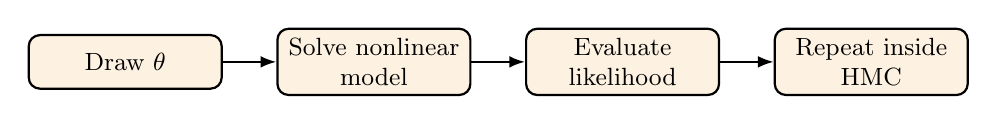
\begin{tikzpicture}[
  node distance=0.68cm,
  box/.style={draw, rounded corners, thick, align=center, font=\small, minimum height=0.68cm, minimum width=2.45cm},
  arr/.style={-{Latex[length=2mm]}, thick}
]
\node[box, fill=PaleOrange] (theta) {Draw $\theta$};
\node[box, fill=PaleOrange, right=of theta] (solve) {Solve nonlinear\\ model};
\node[box, fill=PaleOrange, right=of solve] (filter) {Evaluate\\ likelihood};
\node[box, fill=PaleOrange, right=of filter] (hmc) {Repeat inside\\ HMC};
\draw[arr] (theta) -- (solve);
\draw[arr] (solve) -- (filter);
\draw[arr] (filter) -- (hmc);
\end{tikzpicture}

\vspace{0.15em}
\footnotesize Repeated many times inside HMC.
\end{center}

\vspace{0.45em}
\textbf{The nested-loop bottleneck}

\softline
\begin{center}
\[
  \theta
  \longmapsto
  g^{\sep}_{\theta}
  \longmapsto
  p(\obs_{1:T}\mid\theta)
  \longmapsto
  \text{MCMC proposal}
\]
\end{center}
The expensive object is recomputed exactly where the sampler needs speed.
\sourcefoot{Benchmark approaches put nonlinear filtering or solution work inside the likelihood loop; see Fern\'andez-Villaverde--Rubio-Ram\'irez (2007), Fern\'andez-Villaverde--Rubio-Ram\'irez--Schorfheide (2016), and Herbst--Schorfheide (2016).}
\end{frame}

% -----------------------------------------------------------------------------
\begin{frame}{The Solution in One Picture}
\claim{The likelihood switches across a solution ladder, not across models.}

\vspace{0.2em}
\begin{columns}[T,onlytextwidth]
\begin{column}{0.43\textwidth}
\centering
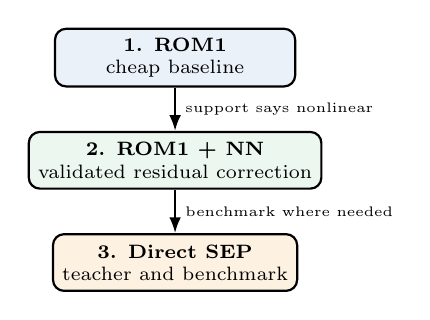
\begin{tikzpicture}[
  node distance=0.55cm,
  box/.style={draw, rounded corners, thick, align=center, minimum height=0.72cm, minimum width=3.05cm, font=\scriptsize},
  arr/.style={-{Latex[length=2mm]}, thick}
]
\node[box, fill=PaleBlue] (rom) {\textbf{1. ROM1}\\ cheap baseline};
\node[box, fill=PaleGreen, below=of rom] (nn) {\textbf{2. ROM1 + NN}\\ validated residual correction};
\node[box, fill=PaleOrange, below=of nn] (sep) {\textbf{3. Direct SEP}\\ teacher and benchmark};
\draw[arr] (rom) -- node[right,font=\tiny] {support says nonlinear} (nn);
\draw[arr] (nn) -- node[right,font=\tiny] {benchmark where needed} (sep);
\end{tikzpicture}
\end{column}
\begin{column}{0.53\textwidth}
\textbf{At each likelihood date}
\[
  \widehat g_t
  =
  g^{\rom}_{\theta}
  +
  \omega(d_t)\,r_{\phi}(\state_t,\eps_{t+1},\theta).
\]

\vspace{-0.4em}
\begin{itemize}
  \item \(d_t\) summarizes support, inversion, and regime diagnostics.
  \item \(\omega(d_t)\approx0\): ROM1 dominates.
  \item \(\omega(d_t)\approx1\): nonlinear residual is active.
  \item Outside validated support: flag the draw or benchmark with direct SEP.
\end{itemize}
\end{column}
\end{columns}

\smallnote{The object is a switching solution-order likelihood. The posterior tells us when first-order dynamics suffice and when nonlinear solution information matters.}
\end{frame}

% -----------------------------------------------------------------------------
\begin{frame}{Algorithm: Switching Solution-Order Likelihood}
\claim{The algorithm is a likelihood evaluator with an observed solution-order switch.}

\vspace{0.15em}
\scriptsize
\begin{table}
\centering
\begin{tabular}{@{}p{0.09\linewidth}p{0.42\linewidth}p{0.39\linewidth}@{}}
\toprule
Stage & Operation & Comparison to related methods \\
\midrule
Offline 1 & Solve SEP at design triples \((\state,\eps,\theta)\). & SEP teacher, not an online likelihood engine. \\
Offline 2 & Compute ROM1 at identical triples and train \(r_\phi\approx g^\sep-g^\rom\). & Residual surrogate, not a full policy-function or likelihood surrogate. \\
Online 1 & Given \(\theta\), invert or sample shocks and compute support score \(d_t\). & Filter-free shock treatment follows Childers et al.; inversion gives the medium-scale profile target. \\
Online 2 & Evaluate \(\widehat g_t=g^\rom_\theta+\omega(d_t)r_\phi\). & Solution order switches by date: ROM1 unless validated nonlinear correction is supported. \\
Online 3 & Accumulate likelihood and use HMC/NUTS on the differentiable target. & HMC sees one smooth target plus diagnostics on where nonlinear information enters. \\
\bottomrule
\end{tabular}
\end{table}

\sourcefoot{Related methods: Fair--Taylor (1983) and Adjemian--Juillard (2013, 2025) for SEP; Childers et al. (2022) for filter-free HMC; Kase--Melosi--Rottner (2025) for neural-network surrogate estimation.}
\end{frame}

% -----------------------------------------------------------------------------
\begin{frame}{What Exactly Is Approximated?}
\claim{The neural net approximates the solved transition map, not the model equations.}

\vspace{0.35em}
\begin{columns}[T,onlytextwidth]
\begin{column}{0.49\textwidth}
\textbf{Equilibrium discipline}
\[
  F(\state_{t-1},\state_t,\state_{t+1},\eps_t;\theta)=0
\]
is imposed by SEP offline, including expectations and constraints.

\vspace{0.5em}
\textbf{Training object}
\[
  g^{\sep}_{\theta}(\state_t,\eps_{t+1})
  =
  \state_{t+1}^{\sep}.
\]
\end{column}
\begin{column}{0.47\textwidth}
\textbf{Residual target}
\[
  r_{\phi}(\state,\eps,\theta)
  \approx
  g^{\sep}_{\theta}(\state,\eps)
  -
  g^{\rom}_{\theta}(\state,\eps).
\]

\vspace{0.5em}
\textbf{Online map}
\[
  \widehat g_{\theta,\phi}
  =
  g^{\rom}_{\theta}
  +
  \omega(\state,\eps,\theta)r_{\phi}.
\]
\end{column}
\end{columns}

\vspace{0.45em}
\begin{center}
\small This distinction matters for econometrics: the approximation is a controlled change to the likelihood, not a new behavioral model.
\end{center}
\sourcefoot{Relative to deep equilibrium nets and NN policy-function solvers (Maliar--Maliar--Winant, 2021; Azinovic--Gaegauf--Scheidegger, 2022), the network here emulates the SEP-implied transition residual used by the likelihood.}
\end{frame}

% -----------------------------------------------------------------------------
\begin{frame}{How the Switching Rule Operates}
\claim{The gate chooses the solution order period by period.}

\vspace{0.15em}
\begin{center}
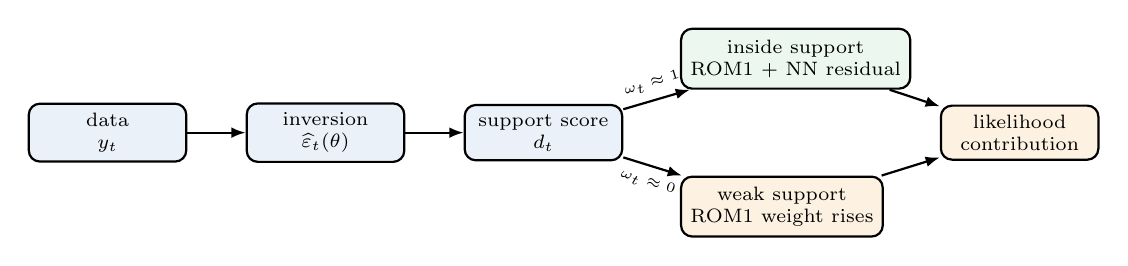
\begin{tikzpicture}[
  node distance=0.54cm and 0.74cm,
  box/.style={draw, rounded corners, thick, align=center, font=\scriptsize, minimum height=0.64cm, minimum width=2.0cm},
  wide/.style={draw, rounded corners, thick, align=center, font=\scriptsize, minimum height=0.76cm, minimum width=2.55cm},
  arr/.style={-{Latex[length=1.8mm]}, thick},
  soft/.style={-{Latex[length=1.8mm]}, thick, dashed}
]
\node[box, fill=PaleBlue] (data) {data\\ $\obs_t$};
\node[box, fill=PaleBlue, right=of data] (inv) {inversion\\ $\widehat{\eps}_t(\theta)$};
\node[box, fill=PaleBlue, right=of inv] (dist) {support score\\ $d_t$};
\node[wide, fill=PaleGreen, above right=0.18cm and 0.72cm of dist] (nn) {inside support\\ ROM1 $+$ NN residual};
\node[wide, fill=PaleOrange, below right=0.18cm and 0.72cm of dist] (romonly) {weak support\\ ROM1 weight rises};
\node[box, fill=PaleOrange] (like) at ($(nn.east)!0.5!(romonly.east)+(1.55,0)$) {likelihood\\ contribution};
\draw[arr] (data) -- (inv);
\draw[arr] (inv) -- (dist);
\draw[arr] (dist) -- node[above, sloped, font=\tiny] {$\omega_t \approx 1$} (nn);
\draw[arr] (dist) -- node[below, sloped, font=\tiny] {$\omega_t \approx 0$} (romonly);
\draw[arr] (nn) -- (like);
\draw[arr] (romonly) -- (like);
\end{tikzpicture}
\end{center}

\vspace{0.05em}
\begin{columns}[T,onlytextwidth]
\begin{column}{0.50\textwidth}
\small
\textbf{Switching transition map}
\[
  \widehat g_t =
  g^{\rom}_{\theta}
  + \omega_t r_{\phi},
  \qquad
  0\leq \omega_t\leq 1 .
\]
\end{column}
\begin{column}{0.46\textwidth}
\small
\textbf{What the switch reports}
\begin{itemize}
  \item Where ROM1 is enough.
  \item Where the NN correction is active.
  \item Which periods need direct SEP benchmark checks.
\end{itemize}
\end{column}
\end{columns}

\vspace{-0.05em}
\begin{center}
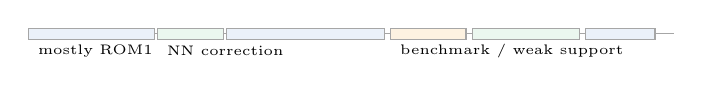
\begin{tikzpicture}[x=0.40cm,y=0.28cm]
\draw[black!35] (0,0) -- (20.5,0);
\foreach \x/\w/\c in {0/4/PaleBlue,4.1/2.1/PaleGreen,6.3/5.0/PaleBlue,11.5/2.4/PaleOrange,14.1/3.4/PaleGreen,17.7/2.2/PaleBlue}
  \draw[fill=\c,draw=black!35] (\x,-0.25) rectangle ++(\w,0.5);
\node[font=\tiny,anchor=west] at (0,-0.78) {mostly ROM1};
\node[font=\tiny,anchor=west] at (4.1,-0.78) {NN correction};
\node[font=\tiny,anchor=west] at (11.5,-0.78) {benchmark / weak support};
\end{tikzpicture}
\end{center}
\end{frame}

% -----------------------------------------------------------------------------
\begin{frame}{Step 0: Choose the Estimation Target}
\claim{Be explicit about the object before approximating it.}

\vspace{0.25em}
\[
  \state_{t+1}=g_\theta(\state_t,\eps_{t+1}),\qquad
  \obs_t=h(\state_t;\theta)+\eta_t,\qquad
  \eps_t\sim\mathcal N(0,I),\quad
  \eta_t\sim\mathcal N(0,\Sigma_y).
\]

\vspace{-0.15em}
\begin{columns}[T,onlytextwidth]
\begin{column}{0.48\textwidth}
\textbf{Objects}
\begin{itemize}
  \item Structural parameters \(\theta\).
  \item State vector \(\state_t\).
  \item Structural shocks \(\eps_t\).
  \item Observables \(\obs_t\).
\end{itemize}
\end{column}
\begin{column}{0.48\textwidth}
\textbf{Choice to make explicit}
\begin{itemize}
  \item Direct measurement-error likelihood or inversion/profile criterion.
  \item Which parameters vary in training and HMC.
  \item Parameter and shock support.
  \item What is benchmarked with direct SEP.
\end{itemize}
\end{column}
\end{columns}

\smallnote{The approximation must be judged relative to this target, not relative to a generic forecast exercise.}
\sourcefoot{The target notation follows the nonlinear state-space estimation tradition in Fern\'andez-Villaverde--Rubio-Ram\'irez (2007), Fern\'andez-Villaverde--Rubio-Ram\'irez--Schorfheide (2016), and Herbst--Schorfheide (2016).}
\end{frame}

% -----------------------------------------------------------------------------
\begin{frame}{Step 1: Solve the Nonlinear Model Offline}
\claim{Use SEP as an offline teacher.}

\vspace{0.2em}
For sampled triples \((\state,\eps,\theta)\), compute the nonlinear transition
\[
  \state^+_{\sep} = g^{\sep}_{\theta}(\state,\eps).
\]

\vspace{-0.15em}
\[
  \E_t m(\state_{t+1})
  \approx
  \sum_{j=1}^{J} w_j\,
  m\!\left(g_\theta^{\sep}(\state_t,\eps_{j,t+1})\right).
\]

\vspace{-0.35em}
\begin{columns}[T,onlytextwidth]
\begin{column}{0.48\textwidth}
\textbf{Why SEP?}
\begin{itemize}
  \item Keeps the nonlinear equations.
  \item Handles occasionally binding constraints.
  \item Gives direct objects for validation.
\end{itemize}
\end{column}
\begin{column}{0.48\textwidth}
\textbf{What must be reported}
\begin{itemize}
  \item Solver tolerances.
  \item Failed and successful points.
  \item Shock and parameter support.
  \item Initialization strategy.
\end{itemize}
\end{column}
\end{columns}
\sourcefoot{SEP builds on Fair--Taylor (1983) and the stochastic extended path implementation of Adjemian--Juillard (2013, 2025). Here SEP is used as an offline teacher and benchmark, not as the repeated likelihood evaluator.}
\end{frame}

% -----------------------------------------------------------------------------
\begin{frame}{Step 2: Compute the Linear Baseline at the Same Points}
\claim{Use the linear solution as the baseline, not as the answer.}

\vspace{0.4em}
At the same inputs, compute
\[
  \state^+_{\rom} = g^{\rom}_{\theta}(\state,\eps).
\]

\vspace{0.4em}
\textbf{Reason}

\softline
The linear solution is cheap and often accurate near the steady state. The NN
should not waste capacity relearning what ROM1 already does well.

\vspace{0.4em}
\begin{center}
\large
\[
  \text{Nonlinear object}
  =
  \text{linear baseline}
  +
  \text{nonlinear correction}.
\]
\end{center}
\sourcefoot{ROM1 uses the perturbation/linear rational-expectations workhorse logic associated with Sims (2002) and the perturbation literature; here it is a control variate and fallback, not the final nonlinear estimator.}
\end{frame}

% -----------------------------------------------------------------------------
\begin{frame}{Step 3: Train the Residual Surrogate}
\claim{Train the nonlinear correction.}

\vspace{0.4em}
Train \(r_{\phi}\) on the residual
\[
  r_{\phi}(\state,\eps,\theta)
  \approx
  g^{\sep}_{\theta}(\state,\eps)
  -
  g^{\rom}_{\theta}(\state,\eps).
\]

\vspace{0.5em}
\begin{columns}[T,onlytextwidth]
\begin{column}{0.48\textwidth}
\textbf{Why residual learning}
\begin{itemize}
  \item Smaller target.
  \item Easier extrapolation around the linear region.
  \item Directly measures what linearization misses.
\end{itemize}
\end{column}
\begin{column}{0.48\textwidth}
\textbf{Resulting transition}
\[
  g_{\phi}(\state,\eps,\theta)
  =
  g^{\rom}_{\theta}(\state,\eps)
  +
  r_{\phi}(\state,\eps,\theta).
\]
\end{column}
\end{columns}
\sourcefoot{Compared with full-map neural solvers (Maliar--Maliar--Winant, 2021; Azinovic--Gaegauf--Scheidegger, 2022) and likelihood surrogates (Kase--Melosi--Rottner, 2025), the target is the smaller ROM1 residual.}
\end{frame}

% -----------------------------------------------------------------------------
\begin{frame}{Step 4: Validate the Surrogate Before Estimation}
\claim{Do not estimate before the surrogate passes basic checks.}

\vspace{0.25em}
\begin{columns}[T,onlytextwidth]
\begin{column}{0.48\textwidth}
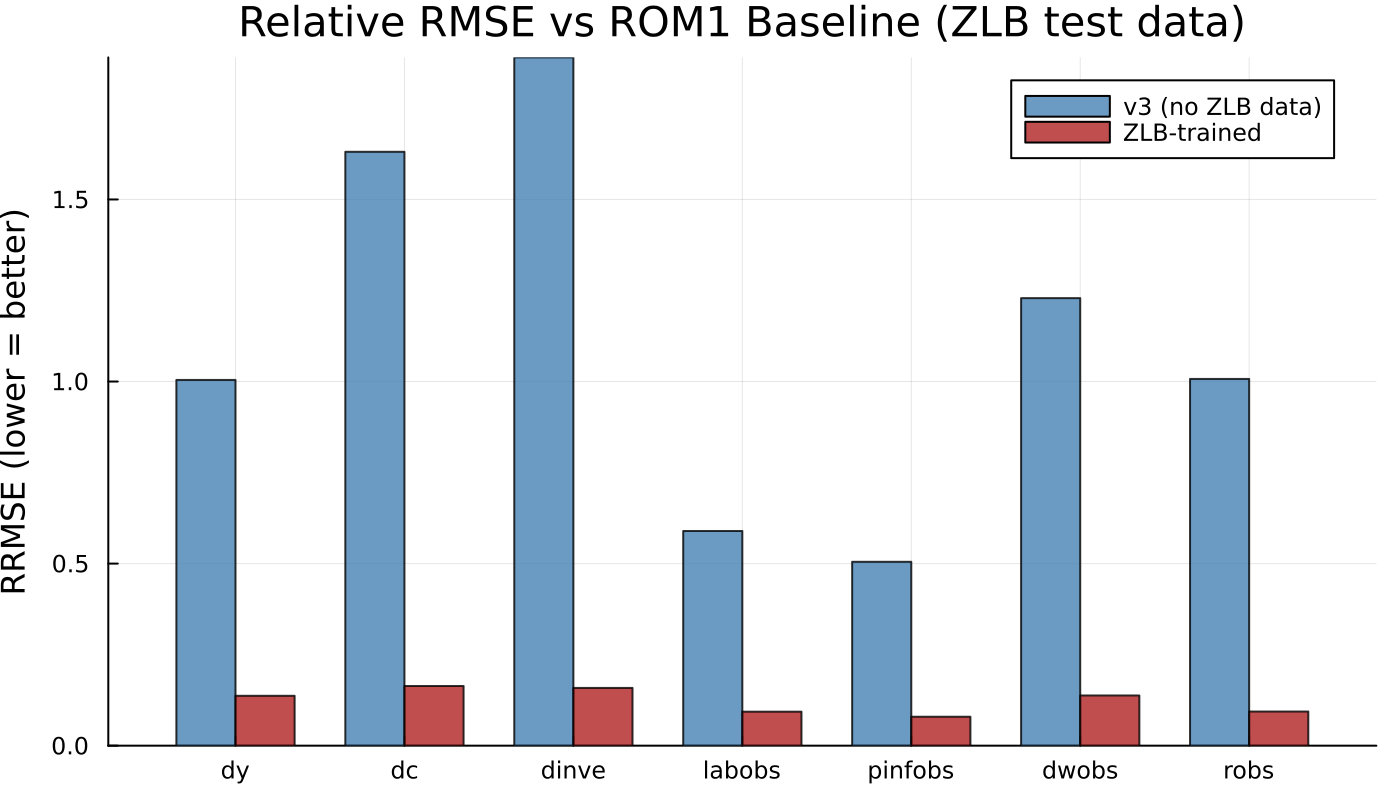
\includegraphics[width=\textwidth,height=0.56\textheight,keepaspectratio]{zlb_rrmse_comparison.png}
\end{column}
\begin{column}{0.48\textwidth}
\textbf{Checks}
\begin{itemize}
  \item Held-out direct SEP points.
  \item RMSE and relative RMSE by observable.
  \item Regime-specific accuracy: binding, non-binding, near-boundary.
  \item Finite likelihood and finite-gradient checks.
\end{itemize}
\vspace{0.25em}
\textbf{Rule}

\softline
The surrogate is only credible on the support where it has been checked.
\end{column}
\end{columns}
\sourcefoot{The validation logic follows surrogate-model practice: out-of-sample errors, support checks, and posterior-level diagnostics; compare Kennedy--O'Hagan (2001), Peherstorfer--Willcox--Gunzburger (2018), and HMC diagnostics in Hoffman--Gelman (2014).}
\end{frame}

% -----------------------------------------------------------------------------
\begin{frame}{Step 5: Build the Likelihood}
\claim{The likelihood determines what the validation has to prove.}

\vspace{0.15em}
\begin{columns}[T,onlytextwidth]
\begin{column}{0.50\textwidth}
\textbf{Direct validation target}
\[
  \state_{t+1}^{m}
  =
  g_\theta^m(\state_t^m,\eps_{t+1}),
  \quad
  m\in\{\sep,\phi\}.
\]
\[
  \ell_m(\theta,\eps_{1:T},\state_0)
  =
  \sum_{t=1}^{T}
  \log \mathcal N
  \!\left(
  \obs_t;h(\state_t^m;\theta),\Sigma_y
  \right).
\]
\scriptsize This is the clean synthetic-data benchmark: direct SEP-HMC versus surrogate-HMC.
\end{column}
\begin{column}{0.46\textwidth}
\textbf{Medium-scale profiled target}
\[
  \widehat{\eps}_{t+1}(\theta)
  =
  I_\theta(\obs_{t+1},\state_t),
\]
\[
  \widehat{\state}_{t+1}
  =
  g^{\rom}_{\theta}(\state_t,\widehat{\eps}_{t+1})
  +
  \omega_t r_{\phi}(\state_t,\widehat{\eps}_{t+1},\theta).
\]
\scriptsize Here inversion fixes shocks period by period; the gate reports when the criterion relies on the nonlinear correction.
\end{column}
\end{columns}
\sourcefoot{The direct validation target uses the filter-free latent-shock formulation of Childers et al. (2022). The profiled target differs from particle/Kalman filtering by recovering shocks period by period and reporting the solution-order switch.}
\end{frame}

% -----------------------------------------------------------------------------
\begin{frame}{Step 6: Sample Parameters with HMC}
\claim{The differentiable surrogate is what makes HMC practical.}

\vspace{0.05em}
\[
  q=(\theta,\state_0,\eps_{1:T}),\qquad
  \log \pi_m(q\mid \obs_{1:T})
  =
  \log p(\theta)+\log p(\state_0\mid\theta)
  +\sum_{t=1}^{T}\log p(\eps_t)+\ell_m(q).
\]

\vspace{-0.35em}
\begin{columns}[T,onlytextwidth]
\begin{column}{0.48\textwidth}
\textbf{What is sampled}
\begin{itemize}
  \item Structural parameters \(\theta\).
  \item Initial condition or state objects.
  \item Latent structural shocks \(\eps_{1:T}\).
  \item Same prior and transforms in direct and surrogate runs.
\end{itemize}
\end{column}
\begin{column}{0.48\textwidth}
\textbf{What HMC checks}
\begin{itemize}
  \item The recursion is differentiable.
  \item Gradients are available through \(\widehat g_t\).
  \item Divergences, energy behavior, and mixing test local geometry.
  \item Matched settings make direct and surrogate posteriors comparable.
\end{itemize}
\end{column}
\end{columns}

\smallnote{The validation standard is posterior agreement within Monte Carlo error, not only a low one-step prediction error.}
\sourcefoot{Filter-free per-period likelihood evaluation follows Childers et al. (2022); NUTS/HMC diagnostics follow Hoffman--Gelman (2014) and Betancourt (2017).}
\end{frame}

% -----------------------------------------------------------------------------
\begin{frame}{Diagnostics: Report What the Switch Uses}
\claim{Diagnostics are reporting requirements, not a separate estimator step.}

\vspace{0.35em}
\begin{table}
\centering
\small
\begin{tabular}{lll}
\toprule
Object & Question & Failure mode \\
\midrule
SEP support & Did the solver cover the region? & Hidden selection \\
Surrogate fit & Is the map accurate where used? & Biased likelihood \\
Gradients & Are target derivatives finite? & Bad HMC geometry \\
HMC chains & Do chains mix and agree? & Unreliable posterior \\
Direct SEP checks & Does SEP confirm key cells? & Unsupported extrapolation \\
\bottomrule
\end{tabular}
\end{table}

\vspace{0.4em}
\begin{center}
\small The replication package should make these checks mechanical, not narrative.
\end{center}
\sourcefoot{These diagnostics distinguish the method from black-box neural estimation: the likelihood reports support, residual error, gradients, HMC behavior, and direct SEP checks where feasible.}
\end{frame}

\begin{frame}{Validation: A Hard Nonlinearity}
\claim{The validation needs a region where linearization actually fails.}

\vspace{-0.05em}
\begin{center}
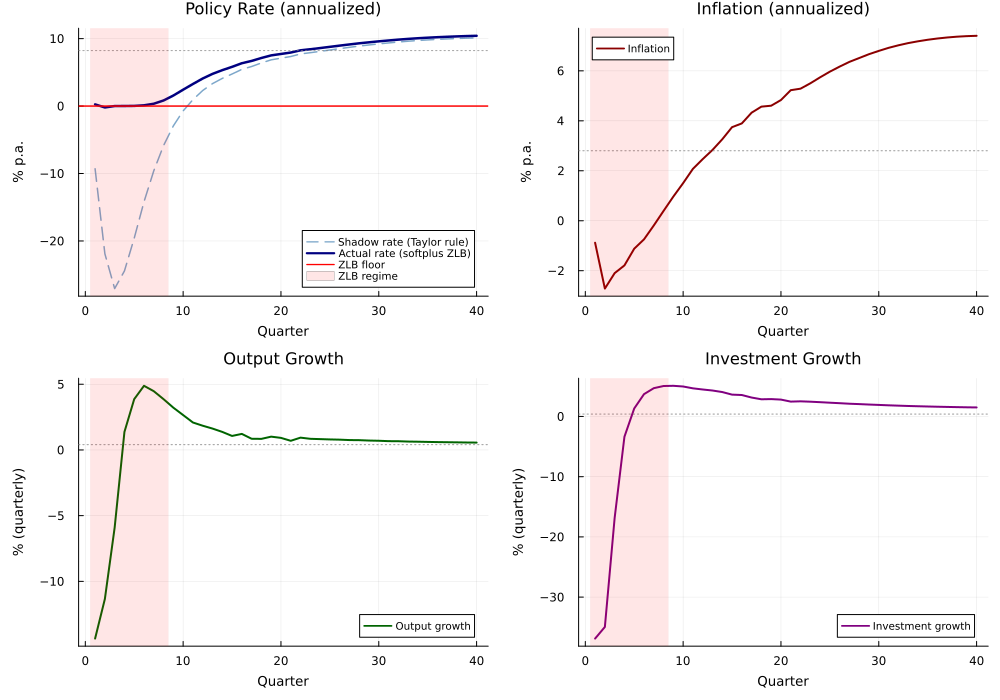
\includegraphics[width=0.84\textwidth,height=0.62\textheight,keepaspectratio]{fig_zlb_binding_simulation.png}
\end{center}
\sourcefoot{Same shocks, nonlinear occasionally-binding model versus linearized model.}
\end{frame}

% -----------------------------------------------------------------------------
\begin{frame}{Validation: Same Inputs, Three Objects}
\claim{A convincing validation holds the shock, state, and parameter vector fixed.}

\vspace{0.15em}
\begin{center}
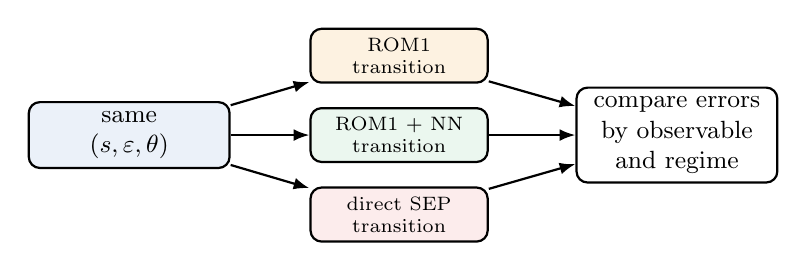
\begin{tikzpicture}[
  node distance=0.7cm and 0.95cm,
  box/.style={draw, rounded corners, thick, align=center, font=\small, minimum height=0.72cm, minimum width=2.55cm},
  smallbox/.style={draw, rounded corners, thick, align=center, font=\scriptsize, minimum height=0.60cm, minimum width=2.25cm},
  arr/.style={-{Latex[length=2mm]}, thick}
]
\node[box, fill=PaleBlue] (input) {same\\ $(\state,\eps,\theta)$};
\node[smallbox, fill=PaleOrange, above right=0.22cm and 1.0cm of input] (rom) {ROM1\\ transition};
\node[smallbox, fill=PaleGreen, right=1.0cm of input] (nn) {ROM1 + NN\\ transition};
\node[smallbox, fill=PaleRed, below right=0.22cm and 1.0cm of input] (sepnode) {direct SEP\\ transition};
\node[box, fill=white, right=1.1cm of nn] (compare) {compare errors\\ by observable\\ and regime};
\draw[arr] (input) -- (rom);
\draw[arr] (input) -- (nn);
\draw[arr] (input) -- (sepnode);
\draw[arr] (rom) -- (compare);
\draw[arr] (nn) -- (compare);
\draw[arr] (sepnode) -- (compare);
\end{tikzpicture}
\end{center}

\vspace{0.2em}
\begin{columns}[T,onlytextwidth]
\begin{column}{0.49\textwidth}
\textbf{Accuracy question}
\[
  \|g^{\sep}-[g^{\rom}+r_{\phi}]\|
  \ll
  \|g^{\sep}-g^{\rom}\|.
\]
\end{column}
\begin{column}{0.47\textwidth}
\textbf{Econometric question}
\[
  p_{\phi}(\theta\mid y_{1:T})
  \approx
  p_{\sep}(\theta\mid y_{1:T}).
\]
\end{column}
\end{columns}

\begin{center}
\parbox{0.90\linewidth}{\centering\scriptsize This is why I report solver support, held-out residuals, finite gradients, HMC diagnostics, and direct SEP posterior comparisons separately.}
\end{center}
\end{frame}

% -----------------------------------------------------------------------------
\begin{frame}{Validation: What the Small Model Shows}
\claim{The small model is a controlled benchmark for the likelihood pipeline.}

\vspace{0.4em}
\begin{columns}[T,onlytextwidth]
\begin{column}{0.48\textwidth}
\textbf{Design}
\begin{itemize}
  \item Nonlinear New Keynesian prototype.
  \item Synthetic data generated by the nonlinear model.
  \item Selected shock-scale parameters estimated.
  \item Direct SEP-HMC compared to surrogate-HMC.
\end{itemize}
\end{column}
\begin{column}{0.48\textwidth}
\textbf{Interpretation}
\begin{itemize}
  \item The pipeline can recover parameters in a controlled nonlinear setting.
  \item The validation is local to the model and support.
  \item It is a feasibility proof, not a universal theorem.
\end{itemize}
\end{column}
\end{columns}
\sourcefoot{The medium-scale laboratory follows the Smets--Wouters tradition and the nonlinear/ZLB estimation literature around Gust--Herbst--L\'opez-Salido--Smith (2017). Results on this slide are preliminary diagnostics.}
\end{frame}

% -----------------------------------------------------------------------------
\begin{frame}{Preliminary Application: Smets--Wouters}
\claim{The medium-scale model is where the computational problem becomes real.}

\vspace{0.4em}
\textbf{Empirical laboratory}

\softline
Smets--Wouters style model with investment adjustment costs, variable
utilization, Kimball pricing and wages, and occasionally binding constraints.

\vspace{0.4em}
\begin{columns}[T,onlytextwidth]
\begin{column}{0.48\textwidth}
\textbf{Why this is useful}
\begin{itemize}
  \item Standard empirical DSGE laboratory.
  \item Rich enough to stress nonlinear mechanisms.
  \item Economically interpretable diagnostic shifts.
\end{itemize}
\end{column}
\begin{column}{0.48\textwidth}
\textbf{Why this is hard}
\begin{itemize}
  \item Higher-dimensional state.
  \item Fragile nonlinear solves.
  \item Strong need for out-of-support diagnostics.
\end{itemize}
\end{column}
\end{columns}
\end{frame}

% -----------------------------------------------------------------------------
\begin{frame}{Preliminary HLT Evidence}
\claim{Near the posterior region, the largest local curvature is on the real side.}

\vspace{-0.05em}
\begin{center}
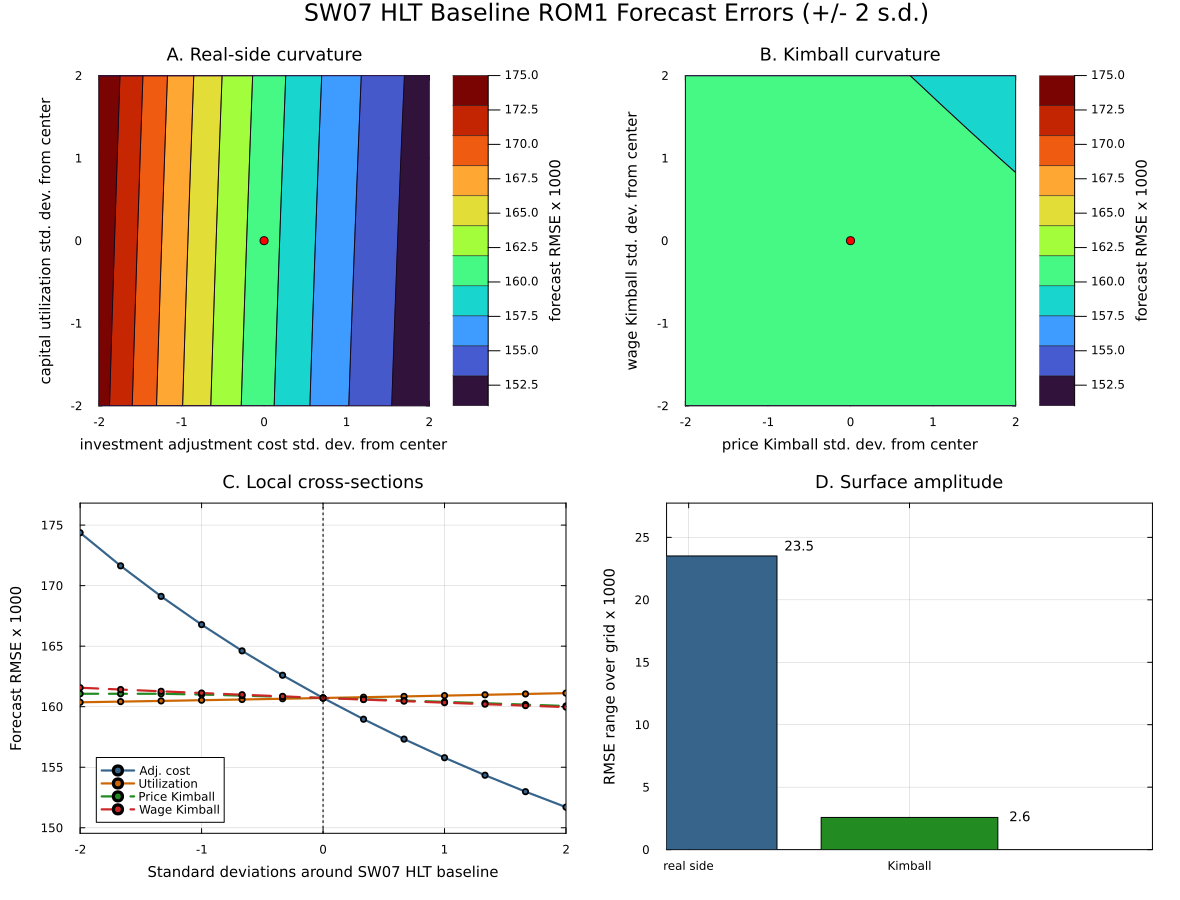
\includegraphics[width=0.84\textwidth,height=0.60\textheight,keepaspectratio]{fig_hlt_curvature_surface_sw07_hlt_baseline_13x13_std2_shock01.png}
\end{center}
\sourcefoot{Preliminary diagnostic evidence: investment and utilization curvature move the SEP--ROM1 forecast error more than Kimball curvature around this posterior-region neighborhood.}
\end{frame}

% -----------------------------------------------------------------------------
\begin{frame}{Preliminary Stress Test: Kimball Can Matter Away From the Posterior Region}
\claim{Kimball curvature can dominate after moving to a deliberately high-curvature neighborhood.}

\vspace{0.35em}
\begin{columns}[T,onlytextwidth]
\begin{column}{0.48\textwidth}
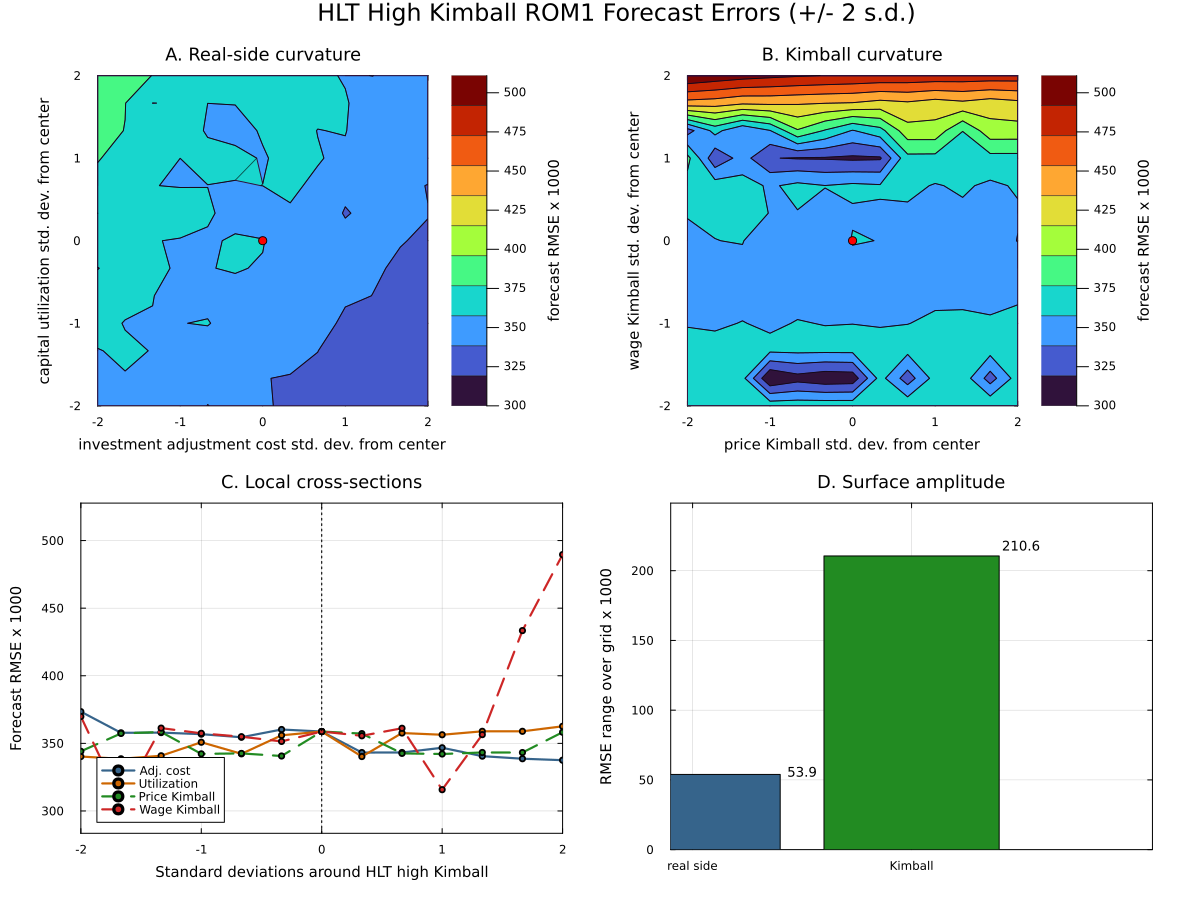
\includegraphics[width=\textwidth,height=0.60\textheight,keepaspectratio]{fig_hlt_curvature_surface_highkimball_13x13_std2_shock01.png}
\end{column}
\begin{column}{0.48\textwidth}
\textbf{What changes}

\softline
If the calibration is deliberately moved to a high price/wage-curvature
neighborhood, Kimball curvature can dominate the local forecast-error surface.

\vspace{0.55em}
\textbf{What this means}

\softline
The investment-channel diagnostic is a posterior-region finding, not a global
claim about every DSGE calibration.
\end{column}
\end{columns}
\end{frame}

% -----------------------------------------------------------------------------
\begin{frame}{Computational Accounting}
\claim{The computational gain is a switched target with amortized nonlinear solves.}

\vspace{0.35em}
\begin{table}
\centering
\small
\begin{tabular}{lcc}
\toprule
Task & Solution order & Role \\
\midrule
SEP solves & benchmark order & expensive teacher \\
ROM1 solution & first order & cheap default \\
ROM1 + NN residual & switched-in order & nonlinear correction \\
Gate/support rule & estimator & chooses order by date \\
HMC & posterior sampler & explores switched target \\
\bottomrule
\end{tabular}
\end{table}

\vspace{0.55em}
\begin{center}
\normalsize The win is not only offline versus online.\\
The win is that the estimator changes solution order only where support has been checked.
\end{center}
\end{frame}

\begin{frame}{Preliminary Evidence: What the Diagnostics Say}
\claim{The evidence is preliminary, but the diagnostics are informative.}

\vspace{0.45em}
\begin{columns}[T,onlytextwidth]
\begin{column}{0.50\textwidth}
\textbf{Method diagnostics}
\begin{itemize}
  \item Corrected unit-shock HLT MVP: 3,200 direct SEP training points.
  \item ROM1-residual NN cuts observable residual RMSE by 87--94 percent.
  \item Small-model ELB/OBC matched HMC diagnostics.
  \item Reduced HLT bridge grid: direct SEP, ROM1, and surrogate surfaces.
  \item Full-NN and linear+gate MVP HMC smokes run without divergences.
\end{itemize}
\end{column}
\begin{column}{0.46\textwidth}
\textbf{Interpretation}
\begin{itemize}
  \item The switching likelihood is operational in controlled settings.
  \item The medium-scale evidence should be read as diagnostic, not final.
  \item The full 18-parameter production posterior is still being extended.
  \item The relevant question is posterior-region support, not average fit.
\end{itemize}
\end{column}
\end{columns}
\end{frame}

% -----------------------------------------------------------------------------
\begin{frame}{Closing Takeaways}
\claim{The method is promising because the approximation is explicit and checkable.}

\vspace{0.35em}
\begin{enumerate}
  \item The computational obstacle is clear: global nonlinear solves are too
        expensive for the inner likelihood loop.
  \item The proposed solution is simple: use ROM1 first, switch in the learned
        SEP residual where support has been checked, and keep direct SEP as the benchmark.
  \item The small nonlinear validation checks posterior agreement, not only fit.
  \item The preliminary Smets--Wouters evidence is useful because it is tied to
        solver support, residual errors, gradients, and HMC diagnostics.
\end{enumerate}

\smallnote{For this audience, the main object is not a black-box NN. It is a likelihood whose solution order is observed, gated, and benchmarked.}
\end{frame}

% -----------------------------------------------------------------------------
\begin{frame}
\begin{center}
\Large Thank you

\vspace{1em}
\normalsize Questions and comments welcome.
\end{center}
\end{frame}

% -----------------------------------------------------------------------------
\appendix

\begin{frame}{Backup: Relation to Gust et al. and MKR}
\small
\begin{table}
\centering
\begin{tabular}{@{}>{\raggedright\arraybackslash}p{0.24\linewidth}>{\raggedright\arraybackslash}p{0.32\linewidth}>{\raggedright\arraybackslash}p{0.34\linewidth}@{}}
\toprule
Approach & What is approximated? & How inference is done \\
\midrule
Gust et al. style OBC estimation & Policy functions with fixed projection basis and regime handling & Particle-filter likelihood and particle-filter MCMC \\
Kase--Melosi--Rottner & Neural-network objects over states and parameters & Fast estimation after offline amortization \\
\textbf{This deck} & \textbf{SEP transition residual over ROM1} & \textbf{Differentiable switched likelihood for HMC} \\
\bottomrule
\end{tabular}
\end{table}

\vspace{0.45em}
\begin{center}
\small The shared idea is amortization. The distinction is the likelihood object: I train a ROM1 residual against direct SEP and report posterior-support checks explicitly.
\end{center}
\end{frame}

% -----------------------------------------------------------------------------
\begin{frame}{Backup: Runtime Budget}
\claim{On this workstation, budget about one week for the production run.}

\vspace{0.2em}
\scriptsize
\begin{table}
\centering
\begin{tabular}{p{0.25\linewidth}p{0.34\linewidth}p{0.29\linewidth}}
\toprule
Component & Measured anchor & Production budget \\
\midrule
Base SEP data & 1,664 corrected unit-shock samples in 2.8 hours & 2--4 days for 125 parameter blocks at longer sample and horizon \\
ZLB SEP data & 1,536 binding samples in 6.3 hours & 2--5 days to obtain about 5,000 accepted binding points \\
Combine and train & 3,200 points trained quickly; NN lowers ROM1 residual RMSE by 87--94 percent & Less than 2 hours unless the dataset is much larger \\
Surrogate HMC & 100 warmup + 100 draws in 25 minutes at tree depth 5 & 3--8 hours per 1,500-iteration chain \\
\bottomrule
\end{tabular}
\end{table}

\vspace{0.25em}
\small If base and ZLB jobs run in parallel, the end-to-end wall-clock estimate is
\textbf{5--8 days}, including training and matched HMC checks.
\end{frame}

% -----------------------------------------------------------------------------
\begin{frame}{Backup: Target and Surrogate Error}
\[
  e_{\phi}(\state,\eps,\theta)
  =
  g^{\sep}_{\theta}(\state,\eps)
  -
  \left[
    g^{\rom}_{\theta}(\state,\eps)
    +
    r_{\phi}(\state,\eps,\theta)
  \right].
\]

\vspace{0.5em}
\begin{block}{Validation quantity}
\[
  \mathrm{RMSE}_{\mathrm{val}}
  =
  \left(
  \frac{1}{N}\sum_{i=1}^{N}
  \| e_{\phi}(\state_i,\eps_i,\theta_i) \|^2
  \right)^{1/2}.
\]
\end{block}

\begin{center}
\small The same held-out inputs are evaluated under direct SEP, ROM1, and the surrogate.
\end{center}
\end{frame}

% -----------------------------------------------------------------------------
\begin{frame}{Backup: Matched HMC Validation Design}
\begin{itemize}
  \item Same synthetic data.
  \item Same prior and parameter transforms.
  \item Same initial values and random seeds.
  \item Same NUTS settings: warmup, draws, target acceptance, tree depth.
  \item Compare posterior means, MCSEs, and 90 percent intervals.
\end{itemize}

\vspace{0.5em}
\begin{block}{Pass criterion}
The surrogate posterior should overlap the direct SEP posterior within Monte
Carlo uncertainty, with no systematic directional distortion.
\end{block}
\end{frame}

% -----------------------------------------------------------------------------
\begin{frame}{Backup: Why SEP?}
\begin{itemize}
  \item Keeps the original nonlinear equations.
  \item Handles occasionally binding constraints directly.
  \item Produces a simulation object that can be compared with perturbation.
  \item Expensive, but parallel over training points.
\end{itemize}

\vspace{0.5em}
\begin{block}{Tradeoff}
SEP is a good offline teacher, but a poor online likelihood engine.
\end{block}
\end{frame}

% -----------------------------------------------------------------------------
\begin{frame}{Backup: Posterior Interpretation}
\begin{itemize}
  \item The small-model validation targets direct likelihood comparisons.
  \item The medium-scale empirical exercise uses an inversion/profiled criterion.
  \item Surrogate HMC results should be read as criterion-based posterior
        diagnostics until a full direct-SEP HMC benchmark is feasible.
\end{itemize}

\vspace{0.5em}
\begin{center}
\small The method is promising because the validation pieces work, not because every medium-scale empirical caveat is already solved.
\end{center}
\end{frame}

\end{document}
